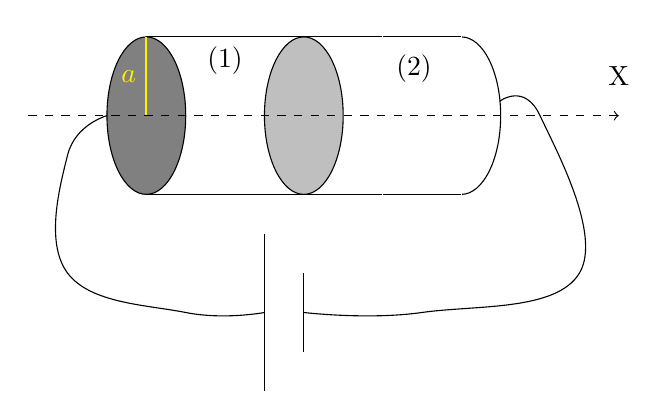
\begin{tikzpicture}

\draw [fill=gray] (-1,0.5) node (v5) {} ellipse (0.5 and 1);
\draw  (3,0.5) node (v1) {} ellipse (0.5 and 1);
\draw [fill=lightgray] (1,0.5) ellipse (0.5 and 1);
\draw (-1,1.5) node (v6) {} -- (3,1.5) node (v3) {};
\draw (-1,-0.5) -- (3,-0.5) node (v2) {};
\draw  plot[smooth, tension=.7] coordinates {(-1.5,0.5) (-2,0) (-2,-1.5) (-0.5,-2) (0.5,-2)};
\draw (0.5,-1) -- (0.5,-3);
\draw (1,-1.5) -- (1,-2.5);
\draw  plot[smooth, tension=.7] coordinates {(1,-2) (2.5,-2) (4.5,-1.5) (4,0.5) (3.4876,0.6831)};
\draw [fill, white] (2,1.5) node (v4) {} rectangle (v2);
\draw (v3.center) -- (v4.center) (v2.center) -- (2,-0.5);
\draw [thick, yellow](v5.center) -- (v6.center) node [midway, left]{$a$};
\draw [->, dashed](-2.5,0.5) -- (5,0.5);
\node at (5,1) {X};
\node at (0,1.2) {(1)};
\node at (2.4,1.1) {(2)};
\end{tikzpicture}